\documentclass[12pt]{article}
\usepackage{geometry}
\usepackage{parskip} % Mengatur jarak antar paragraf tanpa indentasi
\usepackage{graphicx}
\usepackage{titlesec}
\usepackage{listings} % Untuk menampilkan kode
\usepackage{xcolor} % Untuk pewarnaan kode
\usepackage{tikz} % Untuk menggambar diagram
\usetikzlibrary{positioning, arrows.meta}
\usepackage{pdflscape} % Untuk orientasi landscape pada halaman tertentu
\usepackage{amsmath}

\usetikzlibrary{positioning, arrows.meta, shapes.geometric}

% Pengaturan halaman
\geometry{a4paper, margin=1in}

% Pengaturan format judul
\titleformat{\section}{\bfseries\Large}{\thesection.}{1em}{}
\titleformat{\subsection}{\bfseries\large}{\thesubsection}{1em}{}
\titleformat{\subsubsection}{\bfseries\normalsize}{\thesubsubsection.}{1em}{}

% Definisi bahasa C# untuk listings
\lstdefinelanguage{CSharp}{
    language=C,
    morekeywords={abstract, as, base, bool, break, byte, case, catch, char, checked, class, const, continue, decimal, default, delegate, do, double, else, enum, event, explicit, extern, false, finally, fixed, float, for, foreach, goto, if, implicit, in, int, interface, internal, is, lock, long, namespace, new, null, object, operator, out, override, params, private, protected, public, readonly, ref, return, sbyte, sealed, short, sizeof, stackalloc, static, string, struct, switch, this, throw, true, try, typeof, uint, ulong, unchecked, unsafe, ushort, using, virtual, void, volatile, while},
    sensitive=true,
    morecomment=[l]{//},
    morecomment=[s]{/*}{*/},
    morestring=[b]", % Handle strings enclosed in double quotes
}

% Update default lstset for CSharp
\lstset{
    language=CSharp,
    basicstyle=\ttfamily\small,
    keywordstyle=\color{blue},
    commentstyle=\color{gray},
    stringstyle=\color{red},
    breaklines=true,
    frame=single,
    captionpos=b,
    showstringspaces=false % Disable visible spaces in strings
}


\begin{document}

\begin{titlepage}
    \centering
    % Logo UI
    
\includegraphics[width=6cm]{Logo Makara.png} % [Ganti dengan path logo Anda]
    \vspace{1cm}
    
    \centering
    \vspace*{1cm}

    \Huge \textbf{UNIVERSITAS INDONESIA} \\
    \vspace{0.5cm}
    \LARGE \textbf{[Persona: Wrath of Nyx]} \\
    \vspace{1cm}
    \LARGE \textbf{LAPORAN PROYEK GAME RPG BERBASIS COMMAND LINE} \\
    \Large \textbf{(FITUR FONDASI)} \\
    
    \vspace{2cm}

    \Large
    Andi Muhammad Alvin Farhansyah (2306161933) \\
    \vspace{0.5 cm}
    Alexander Christhian (2306267025) \\
    \vspace{0.5 cm}
    Daffa Sayra Firdaus (2306267151) \\
    \vspace{0.5 cm}
    Fathan Yazid Satriani (2306250560) \\
    \vspace{0.5 cm}
    
    \vfill

    \LARGE
    \textbf{Fakultas Teknik} \\
    \textbf{Teknik Komputer} \\
    \textbf{2024} \\
\end{titlepage}


\section{Pendahuluan}
    \subsection{Deskripsi Proyek}
        \textbf{Persona: Wrath of Nyx} merupakan proyek pengembangan \textit{game} bergenre \textit{Role-Playing Game} (RPG) yang dikembangkan oleh kami dari Kelompok L sebagai tugas pasca-UTS untuk mata kuliah Pemrograman Berorientasi Objek (OOP). Permainan ini terinspirasi dari seri game populer \textit{Dark Souls}, sehingga menghadirkan tantangan dengan alur permainan yang mendalam serta mekanisme permainan yang cukup kompleks. Permainan ini dibuat menggunakan Bahasa Pemrograman \textit{C\#} dan dirancang untuk dimainkan melalui antarmuka berbasis teks pada terminal menggunakan \textit{Command-Line Interface} (CLI).
    \subsection{Tujuan Pembelajaran}
        Proyek ini bertujuan untuk:
        \begin{enumerate}
            \item Menerapkan konsep-konsep dasar Pemrograman Berorientasi Objek (OOP) ke dalam proyek pengembangan yang terstruktur dan sistematis.
            \item Mengembangkan serta mengimplementasikan fitur-fitur dasar yang terdapat dalam permainan RPG berbasis command-line.
            \item Mendokumentasikan proses pengembangan dalam bentuk video dan laporan tertulis yang menjelaskan implementasi teknis serta alur logika dari kode yang dirancang.
        \end{enumerate}

\section{Deskripsi Game}    
    \subsection{Deskripsi Singkat}
        \textbf{Persona: Wrath of Nyx} adalah permainan RPG berbasis teks yang mengangkut genre Souls-like Adventure dengan sistem pertarungan berbasis giliran atau dikenal sebagai sistem \textit{turn-based}. Sesuai dengan genre-nya, \textit{Game} ini dirancang untuk tipe pemain yang menyukai tantangan strategis dengan alur cerita yang mendalam.
        Fitur utama permainan ini meliputi:
        \begin{enumerate}
            \item Kemampuan memanggil bantuan dari neraka (\textit{Summon-Based Party Member}).
            \item Sistem XP yang menantang (\textit{Souls-Like Points System}).
            \item Eksplorasi area dengan level klasik.
            \item Pertempuran melawan bos yang sangat epik.
        \end{enumerate}
        Sehingga, permainan ini menghadirkan pengalaman bermain yang menggabungkan strategi, eksplorasi, dan alur cerita yang intens kepada pemainnya.
    \subsection{Alur Cerita}
        Latar cerita permainan ini, berada di dunia yang hampir sepenuhnya ditelan kegelapan akibat kedatangan Nyx, Dewi Malam, yang membawa kehancuran abadi bagi umat manusia. Pemain berperan sebagai Traveler, titisan Thanatos, yang memiliki misi untuk melawan Nyx dan mengembalikan cahaya ke dunia. Dalam perjalanan, Traveler harus mengalahkan musuh-musuh yang menghalangi jalannya ke Istana Nyx. Konflik utama yang dihadapi pemain adalah melawan musuh dari berbagai dimensi dan memanfaatkan kekuatan dewa kematian untuk menghadapi kegelapan yang tak terelakkan.
    \subsection{Gameplay Inti}
        \textit{Gameplay} inti permainan \textbf{Persona: Wrath of Nyx} meliputi:
        \begin{enumerate}
            \item[\textbf{A.}] \textbf{Mekanisme Pertarungan:} Menggunakan sistem \textit{turn-based combat} di mana setiap aksi memiliki peluang keberhasilan yang berbeda, sehingga menciptakan elemen ketidakpastian dalam pertempuran.
            \item[\textbf{B.}] \textbf{Eksplorasi Dunia:} Pemain dapat menjelajahi dunia yang luas dengan berbagai lokasi seperti Istana Nyx, area gua peta, hingga tanah tandus yang penuh misteri. Setiap lokasi memiliki \textit{points of interest} seperti musuh, item, atau interaksi yang berbeda dan unik.
            \item[\textbf{C.}] \textbf{Interaksi dengan Lingkungan serta Musuh:} Pemain dapat bertarung dengan musuh, mengumpulkan item, dan membuka jalur baru yang menuju tujuan akhir. Selain itu, fitur lainnya seperti \textit{random encounter} menambah tantangan selama eksplorasi serta membuat permainan tidak terasa terlalu repetitif.
        \end{enumerate}
    \subsection{Sistem Mekanika}
        Berikut adalah ringkasan dari mekanika permainan \textbf{Persona: Wrath of Nyx}:
        \begin{enumerate}
            \item[\textbf{A.}] \textbf{Pergerakan Karakter:} Karakter pemain dapat berpindah antar area menggunakan sistem eksplorasi berbasis teks. Untuk itu, pemain dapat memilih aksi menggunakan nomor yang sesuai dengan menu pada \textit{interface}.
            \item[\textbf{B.}] \textbf{Interaksi dengan Objek dan Musuh:} Pemain dapat mengakses inventaris (\textit{inventory}) untuk melihat dan melengkapi senjata (\textit{weapon}), baju (\textit{armor}), serta menggunakan item penyembuhan (\textit{healing}) selama pertempuran ataupun ketika eksplorasi.
            \item[\textbf{C.}] \textbf{Penggunaan Item dan Summon:} Sistem inventaris (\textit{inventory}) memungkinkan pemain untuk menggunakan alat seperti obat penyembuh (\textit{healing}) atau memanggil sekutu (\textit{summon ally}) dari neraka, yang diperoleh dengan mengumpulkan fragmen kekuatan Thanatos.
            \item[\textbf{D.}] \textbf{Sistem Level-Up:} XP dalam bentuk Tartarus Essence digunakan untuk meningkatkan level karakter, yang akan meningkatkan statistik pemain seperti kekuatan serangan, pertahanan, dan kesehatan (\textit{health}) maksimum.
        \end{enumerate}
        
\section{Deskripsi Fitur Fondasi}
    \subsection{Sistem Karakter}
        \begin{itemize}
            \item \textbf{Deskripsi Implementasi:}  \\
            Sistem karakter mencakup definisi dan pengelolaan atribut utama untuk pemain, musuh, dan bos dalam permainan. Setiap karakter memiliki atribut seperti HP, serangan, pertahanan, level, dan Tartarus Essence. Pemain juga dapat melengkapi senjata atau armor yang memengaruhi statistik total.
            \item \textbf{Lampiran Kode:}
        \end{itemize}
\begin{lstlisting}[language=CSharp, caption=Implementasi Sistem Karakter]
public class Character
{
    public string Name { get; set; }
    public int HP { get; set; }
    public int MaxHP { get; set; }
    public int Attack { get; set; }
    public int Defense { get; set; }
    public int Level { get; set; }
    public int TartarusEssence { get; set; }
    public int TartarusEssenceOnDeath { get; set; }
    public int TotalAttack => Attack + (EquippedWeapon?.Value ?? 0);
    public int TotalDefense => Defense + (EquippedArmor?.Value ?? 0);

    public Item EquippedWeapon { get; set; }
    public Item EquippedArmor { get; set; }

    public Character(string name, int hp, int attack, int defense)
    {
        Name = name;
        HP = hp;
        MaxHP = hp;
        Attack = attack;
        Defense = defense;
        Level = 1;
        TartarusEssence = 0;
        TartarusEssenceOnDeath = 0;
    }
}
\end{lstlisting}

\subsection{Sistem Lokasi}
\textbf{Deskripsi Implementasi:}  \\
Sistem Location akan mengatur bagaimana perlokasian dari dimana player tersebut berada. Player akan dapat berpindah lokasi dengan masing - masing lokasi akan memiliki beberapa point of interest. Location ini akan memiliki sebuah boss yang dapat dilawan oleh player jika player ingin melawan boss tersebut. 


\textbf{Contoh Implementasi Kode:}
\begin{lstlisting}[language=CSharp, caption=Contoh Implementasi Sistem Location]
public class Location
{
    public string Name { get; set; }
    public bool IsExplored { get; set; }
    public List<PointOfInterest> PointsOfInterest { get; set; }
    public Boss LevelBoss { get; set; }
    public bool IsBossDefeated { get; set; }

    public Location(string name)
    {
        Name = name;
        IsExplored = false;
        PointsOfInterest = new List<PointOfInterest>();
        LevelBoss = null;
        IsBossDefeated = false;
    }
}
\end{lstlisting}

\subsection{Sistem Points of Interest}
\textbf{Deskripsi Implementasi:} \\
Points of Interest adalah bagian dari location yang ada dan akan mengatur enemy, item, dan summon yang ada. Masing - masing point of interest akan memiliki isi - isi yang berbeda dan unik. 

\textbf{Contoh Implementasi Kode:}
\begin{lstlisting}[language=CSharp, caption=Contoh Implementasi Points of Interest]
public class PointOfInterest
{
    public string Name { get; set; }
    public string Description { get; set; }
    public bool IsExplored { get; set; }
    public List<Character> Enemies { get; set; }
    public List<Item> Items { get; set; }
    public List<Summon> Summons { get; set; }

    public PointOfInterest(string name, string description)
    {
        Name = name;
        Description = description;
        IsExplored = false;
        Enemies = new List<Character>();
        Items = new List<Item>();
        Summons = new List<Summon>();
    }
}
\end{lstlisting}

\subsection{Combat System dengan Attack}
\textbf{Deskripsi Implementasi:} \\
Combat System dengan Attack ini akan mengatur core dari combat pada game ini. Combat system yang terpakai akan berupa turn based dimana player akan melakukan attack dahulu lalu dilanjutkan dengan enemy yang akan dilawan. Setiap attack akan dilakukan secara bergantian sampai salah satu entity akan mati (HP < 0). Player dapat memilih untuk antara melakukan attack, defend, atau memakai summon untuk melawan enemy yang ada. Kalkulasi dari damage yang terjadi akan dilakukan dengan hit chance secara random dengan atribut untuk damagenya akan mengikuti dari item - item dan stats dari masing - masing entity yang sedang melakukan combat. Jika player berhasil mengalahkan enemy maka player akan mendapatkan essence berupa experience untuk player yang akan nanti dapat digunakan untuk menaikkan level player.

\textbf{Contoh Implementasi Kode:}
\begin{lstlisting}[language=CSharp, caption=Contoh Implementasi Combat System dengan Attack]
private void InitiateCombat(Character enemy)
        {
            Console.WriteLine($"\nCombat started with {enemy.Name}!");
            Console.WriteLine(ENEMY_SPRITE);
            Console.WriteLine("\nVS\n");
            Console.WriteLine(PLAYER_SPRITE);
            bool playerTurn = true;

            while (enemy.HP > 0 && player.HP > 0)
            {
                if (playerTurn)
                {
                    Console.WriteLine("\nYour turn!");
                    Console.WriteLine("1. Attack");
                    Console.WriteLine("2. Defend");
                    Console.WriteLine("3. Use Summon");

                    string choice = Console.ReadLine();
                    switch (choice)
                    {
                        case "1":
                            Console.WriteLine(@"
                            ⚔️
                             /||\ 
                            ");
                            PerformAttack(player, enemy);
                            break;
                        case "2":
                            Console.WriteLine(@"
                            ��️
                             /||\ 
                            ");
                            player.Defense *= 2; // Temporary defense boost
                            Console.WriteLine($"{player.Name} takes defensive stance!");
                            break;
                        case "3":
                            if (activeParty.Any())
                            {
                                Console.WriteLine(@"
                                ✨
                                \[T]/
                                ");
                                Summon summon = activeParty[0]; // Use first summon for simplicity
                                PerformAttack(summon, enemy);
                            }
                            else
                            {
                                Console.WriteLine("No summons in active party!");
                                continue;
                            }
                            break;
                    }
                }
                else
                {
                    // Enemy turn
                    Console.WriteLine(@"
                    �� Enemy Turn!
                    ");
                    PerformAttack(enemy, player);
                }
                playerTurn = !playerTurn;
            }

            if (enemy.HP <= 0)
            {
                Console.WriteLine(@"
                �� VICTORY!
                ");
                int essence = new Random().Next(10, 30);
                player.TartarusEssence += essence;
                Console.WriteLine($"Victory! Gained {essence} Tartarus Essence");
                if(player.Chance == 1){
                    Console.WriteLine($"And You have reclaimed your Essence");
                    Console.WriteLine($"Don't let them take it away again.");
                }
            }
            else
            {
                Console.WriteLine(@"
                �� DEFEATED
                ");
                Console.WriteLine("You have been defeated...");
                HandlePlayerDeath();
            }
        }

        private void PerformAttack(Character attacker, Character target)
        {
            // Calculate hit chance (70-90%)
            int hitChance = new Random().Next(70, 91);
            if (new Random().Next(1, 101) <= hitChance)
            {
                int damage = Math.Max(1, attacker.TotalAttack - target.Defense);
                target.HP -= damage;
                Console.WriteLine($"{attacker.Name} deals {damage} damage to {target.Name}!");
            }
            else
            {
                Console.WriteLine($"{attacker.Name}'s attack missed!");
            }
        }
\end{lstlisting}


\subsection{Area Movement System}
\textbf{Deskripsi Implementasi:} \\ 
Area movement ini akan mengatur pergerakan dari area - area yang tersedia dalam game ini. Player dapat berpidah dari satu area ke area yang lain untuk mendapatkan pengalaman bermain yang lebih beranekaragam dan menarik. Namun player harus mengalahkan boss terlebih dahulu sebelum melakukan perpindahan ke area selanjutnya. Jika berpindah maka player akan berpindah ke location yang baru bedasarkan location yang telah ada sebelumnya.

\textbf{Contoh Implementasi Kode:}
\begin{lstlisting}[language=CSharp, caption=Contoh Implementasi Area Movement System]
private void MoveToNextArea()
{
    Location currentLocation = currentLevel[currentLocationIndex];
    
    if (!currentLocation.IsBossDefeated)
    {
        Console.WriteLine("You must defeat the boss before moving to the next area!");
        return;
    }

    currentLocationIndex++;
    if (currentLocationIndex >= currentLevel.Count)
    {
        Console.WriteLine("Level complete! Moving to next level...");
        InitializeLevel("Nyx Palace - Next Floor");
        currentLocationIndex = 0;
    }

    Console.WriteLine($"Moved to {currentLevel[currentLocationIndex].Name}");
}
    }

    public class Program
    {
        public static void Main(string[] args)
        {
            Game game = new Game();
            game.StartGame();
        }
    }
}
\end{lstlisting}

\subsection{Boss Fight System}
\textbf{Deskripsi Implementasi:} \\
Sistem boss fight adalah sistem yang memiliki sistem yang mirip dengan combat sistem sebelumnya. Namun pada kali ini enemy yang dilawan adalah boss yang ada pada location tersebut. Boss akan memiliki attack yang berbeda dengan enemy yamg sebelumnya telah dijelaskan. Boss fight ini juga akan mengatur untuk perpindahan ke location lainnya.

\textbf{Contoh Implementasi Kode:}
\begin{lstlisting}[language=CSharp, caption=Contoh Implementasi Boss Fight System]
private void InitiateBossFight(Boss boss)
{
    int tempHP = boss.HP;
    Console.WriteLine($"\n=== BOSS BATTLE ===");
    Console.WriteLine($"Challenging {boss.Name}, {boss.Title}!");
    Console.WriteLine(@"
    �� BOSS BATTLE INITIATED!
    ");

    bool playerTurn = true;

    while (boss.HP > 0 && player.HP > 0)
    {
        if (playerTurn)
        {
            Console.WriteLine($"\nYour turn! Boss HP: {boss.HP}");
            Console.WriteLine("1. Attack");
            Console.WriteLine("2. Defend");
            Console.WriteLine("3. Use Summon");
            Console.WriteLine("4. Use Item");

            string choice = Console.ReadLine();
            switch (choice)
            {
                case "1":
                    PerformAttack(player, boss);
                    break;
                case "2":
                    player.Defense *= 2;
                    Console.WriteLine($"{player.Name} takes defensive stance!");
                    break;
                case "3":
                    if (activeParty.Any())
                    {
                        UseSummonInBattle(boss);
                    }
                    else
                    {
                        Console.WriteLine("No summons in active party!");
                        continue;
                    }
                    break;
                case "4":
                    UseItemInBattle();
                    continue;
            }
        }
        else
        {
            // Boss turn with special moves
            Console.WriteLine($"\n{boss.Name}'s turn!");
            if (new Random().Next(100) < 30)
            {
                // 30% chance for special attack
                int damage = boss.Attack * 2;
                player.HP -= damage;
                Console.WriteLine($"{boss.Name} uses special attack! Deals {damage} damage!");
            }
            else
            {
                PerformAttack(boss, player);
            }
        }
        playerTurn = !playerTurn;
    }

    if (boss.HP <= 0)
    {
        Console.WriteLine(@"
        �� BOSS DEFEATED!
        ");
        int essence = new Random().Next(50, 100);
        player.TartarusEssence += essence;
        Console.WriteLine($"Victory! Gained {essence} Tartarus Essence");
        currentLevel[currentLocationIndex].IsBossDefeated = true;
    }
    else
    {
        Console.WriteLine(@"
        �� DEFEATED BY BOSS
        ");
        boss.HP = tempHP;
        HandlePlayerDeath();
    }
}
\end{lstlisting}

\subsection{Level Up System}
\textbf{Deskripsi Implementasi:} \\
Level up system ini akan mengatur mengenai stats player dimana player dapat menaikkan stats - stats yang ada pada player tersebut jika level player tersebut akan naik. Level dari player tersebut akan diatur oleh essence yang telah dikumpulkan oleh player tersebut dari battle - battle yang ada. Lalu jika player sudah cukup mengumpulkan essence tersebut maka player dapat menaikkan level untuk menaikkan stats yang ada.

\textbf{Contoh Implementasi Kode:}
\begin{lstlisting}[language=CSharp, caption=Contoh Implementasi Boss Fight System]
private void VisitTemple()
        {
            Console.WriteLine("\n=== Temple of Ascension ===");
            Console.WriteLine($"Current Level: {player.Level}");
            Console.WriteLine($"Your Tartarus Essence: {player.TartarusEssence}");
            
            int requiredEssence = 5 * player.Level;
            Console.WriteLine($"\nRequired Essence for next level: {requiredEssence}");
            Console.WriteLine("Benefits per level:");
            Console.WriteLine("- Max HP +10");
            Console.WriteLine("- Attack +2");
            Console.WriteLine("- Defense +1");
            
            Console.WriteLine("\nDo you wish to level up? (Y/N)");
            string choice = Console.ReadLine()?.ToUpper();

            if (choice == "Y")
            {
                if (player.TartarusEssence >= requiredEssence)
                {
                    player.TartarusEssence -= requiredEssence;
                    player.Level++;
                    player.MaxHP += 10;
                    player.HP = player.MaxHP; // Heal to full when leveling up
                    player.Attack += 2;
                    player.Defense += 1;
                    
                    Console.WriteLine($"\nLevel Up! You are now level {player.Level}!");
                    Console.WriteLine($"New Stats:");
                    Console.WriteLine($"HP: {player.HP}/{player.MaxHP}");
                    Console.WriteLine($"Attack: {player.Attack}");
                    Console.WriteLine($"Defense: {player.Defense}");
                }
                else
                {
                    Console.WriteLine("Not enough Tartarus Essence!");
                }
            }
        }
\end{lstlisting}

\section{Penerapan Konsep OOP dan Relasi antar Kelas/Objek}

\textbf{Diagram Kelas:} \\

% Mulai halaman landscape
\begin{landscape}
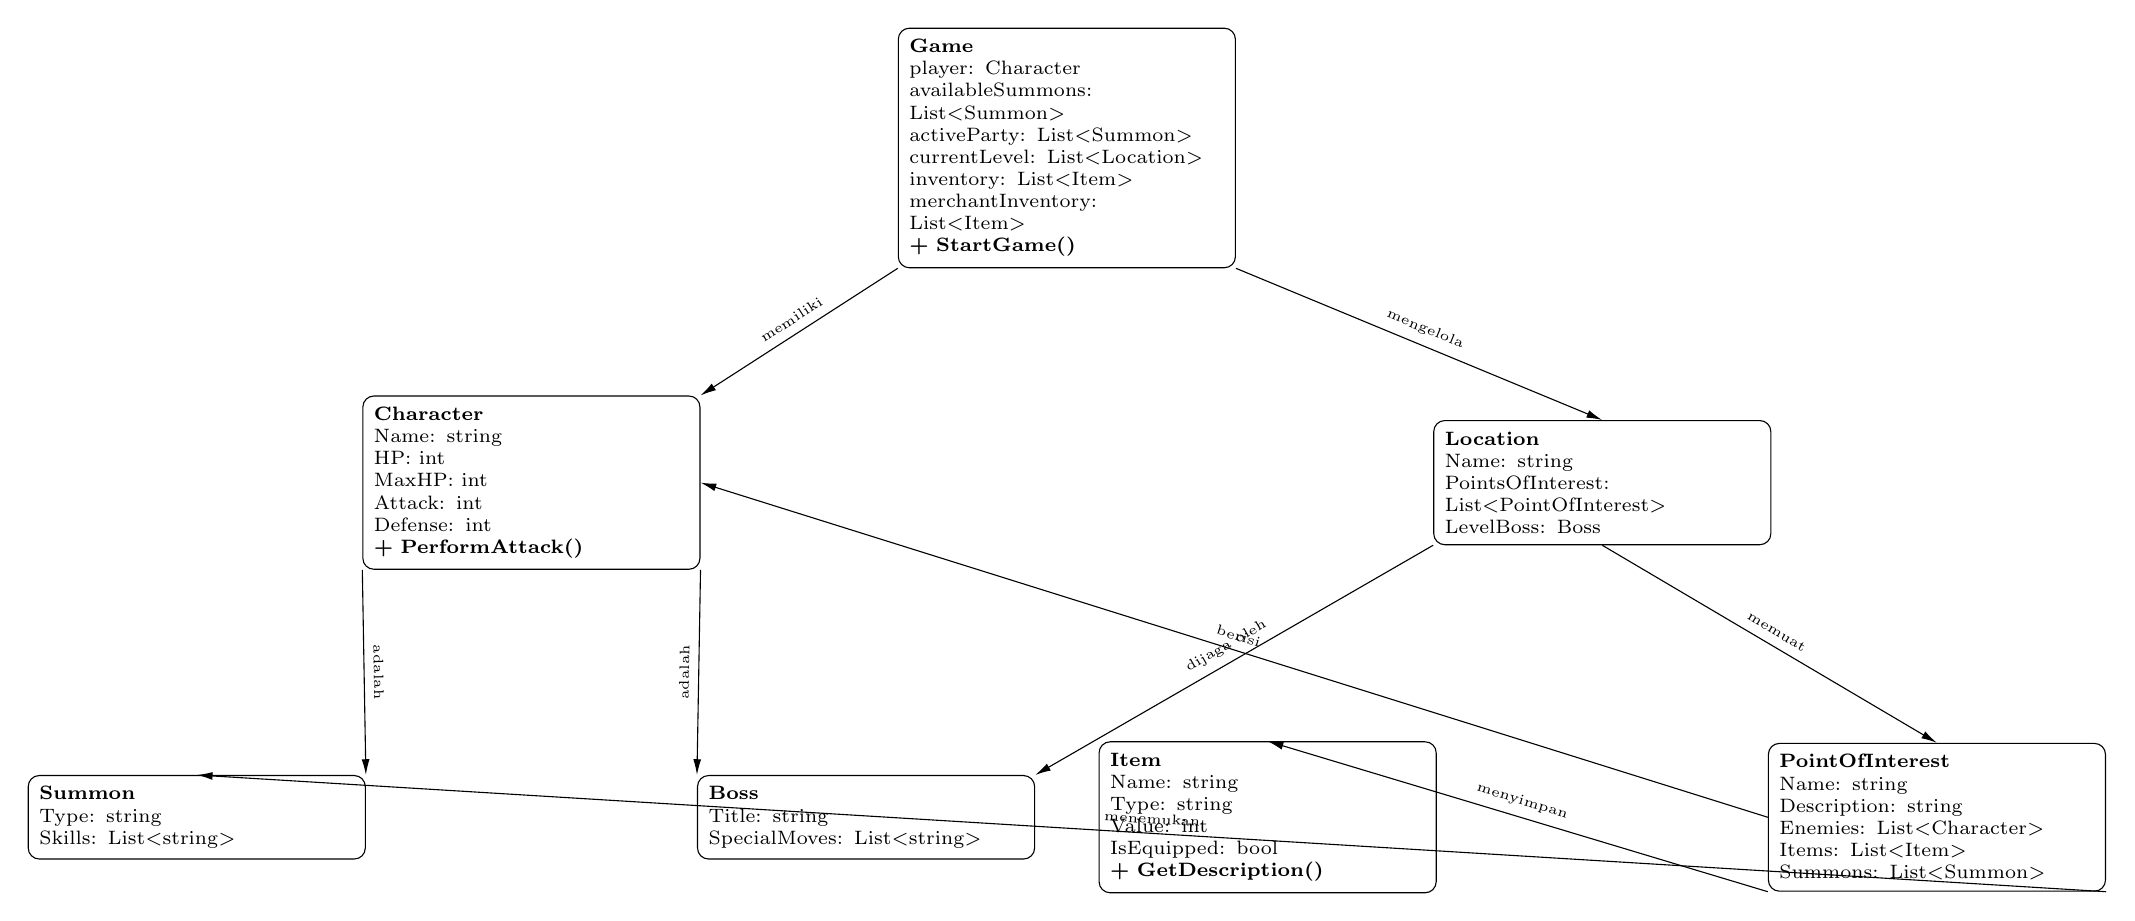
\begin{tikzpicture}[
    font=\scriptsize, % Ukuran font lebih kecil
    scale=0.85, % Mengecilkan seluruh diagram
    every node/.style={scale=1}, % Skalakan semua elemen
    class/.style={rectangle, draw=black, rounded corners, text width=4cm, align=left, minimum height=0.8cm, inner sep=4pt},
    relation/.style={draw, -{Latex[length=2mm, width=1mm]}},
    textrelation/.style={midway, sloped, above, font=\tiny}
]

% Menentukan kelas
\node[class] (game) at (0, 7) {
    \textbf{Game}\\
    player: Character\\
    availableSummons: List$<$Summon$>$\\
    activeParty: List$<$Summon$>$\\
    currentLevel: List$<$Location$>$\\
    inventory: List$<$Item$>$\\
    merchantInventory: List$<$Item$>$\\
    \textbf{+ StartGame()}
};

\node[class] (character) at (-8, 2) {
    \textbf{Character}\\
    Name: string\\
    HP: int\\
    MaxHP: int\\
    Attack: int\\
    Defense: int\\
    \textbf{+ PerformAttack()}
};

\node[class] (summon) at (-13, -3) {
    \textbf{Summon}\\
    Type: string\\
    Skills: List$<$string$>$
};

\node[class] (boss) at (-3, -3) {
    \textbf{Boss}\\
    Title: string\\
    SpecialMoves: List$<$string$>$
};

\node[class] (location) at (8, 2) {
    \textbf{Location}\\
    Name: string\\
    PointsOfInterest: List$<$PointOfInterest$>$\\
    LevelBoss: Boss
};

\node[class] (pointofinterest) at (13, -3) {
    \textbf{PointOfInterest}\\
    Name: string\\
    Description: string\\
    Enemies: List$<$Character$>$\\
    Items: List$<$Item$>$\\
    Summons: List$<$Summon$>$
};

\node[class] (item) at (3, -3) {
    \textbf{Item}\\
    Name: string\\
    Type: string\\
    Value: int\\
    IsEquipped: bool\\
    \textbf{+ GetDescription()}
};

% Relasi antar kelas
\draw[relation] (game.south west) -- node[textrelation] {memiliki} (character.north east);
\draw[relation] (game.south east) -- node[textrelation] {mengelola} (location.north);
\draw[relation] (location.south) -- node[textrelation] {memuat} (pointofinterest.north);
\draw[relation] (location.south west) -- node[textrelation] {dijaga oleh} (boss.north east);
\draw[relation] (pointofinterest.west) -- node[textrelation] {berisi} (character.east);
\draw[relation] (pointofinterest.south west) -- node[textrelation] {menyimpan} (item.north);
\draw[relation] (pointofinterest.south east) -- node[textrelation] {menemukan} (summon.north);
\draw[relation] (character.south west) -- node[textrelation] {adalah} (summon.north east);
\draw[relation] (character.south east) -- node[textrelation] {adalah} (boss.north west);

\end{tikzpicture}
\end{landscape}
% Akhir halaman landscape



\textbf{Penjelasan Relasi:} \\
Relasi ini menjelaskan dari konsep game ini dimana : 
\begin{enumerate}
    \item Game akan memiliki isi character dimana game akan mengelola location
    \item Character ini akan diturunkan menjadi 2 yaitu Boss dan Summon
    \item Location akan memuat Point Of Interest dan akan memiliki atau lokasi tersebut akan dijaga oleh sebuah boss
    \item Point of Interest akan menyimpan item - item dan dapat mengsummon enemy (summon)
\end{enumerate}

\section{Rencana Fitur Tambahan}
\subsection{}
\textbf{Deskripsi Implementasi:} \\


\subsection{Random Encounter}
\textbf{Deskripsi Implementasi:} \\
Dalam map exploration, kita memiliki kesempatan random untuk mendapat encounter battle dengan musuh yang random. Musuh tersebut berupa random, dapat berbentuk undead soldier biasa yang mudah dilawan ataupun miniboss. Persentase encounter akan ditentukan dari lokasi sang pemain berada. Jika berada pada lokasi dimana encounter undead soldier banyak maka persentase undead soldier akan naik dan sebagainya. Random encounter ini juga bisa berupa unique interaction seperti terdapat item baru, buff / efek terhadap status karakter (misalkan tiba-tiba merasa lapar sehingga HP berkurang sekian persen),dll.

\subsection{}
\textbf{Deskripsi Implementasi:} \\

\subsection{Character Creation Preset}
\textbf{Deskripsi Implementasi:} \\
Untuk awal game, terdapat beberapa preset karakter yang bisa dipilih dengan keuntungan dan kerugiannya masing-masing, misalkan Magic-based (Mage) atau Strength-based (Knight) . Karakter ini akan kita progress sehingga dengan Tartarus-Essence bisa digunakan untuk Level Up menaikkan stats karakter player.

\subsection{Gauntlet Mode}
\textbf{Deskripsi Implementasi:} \\
Area khusus yang akan men-spawn musuh-musuh dengan persentase spawn musuh lebih susah akan naik seiring waktu. Area ini seperti sebuah survival mode untuk mendapatkan Tartarus-Essence (poin) secara langsung tanpa harus eksplorasi. Akan tetapi, perlu diingat bahwa player harus tau kapan ia akan berhenti atau melanjutkan mode ini, karena jika karakter kalah, seperti yang disebutkan pada fitur gameplay utama maka Tartarus-Essence dari karakter player akan menghilang dan hanya bisa didapatkan dengan mengalahkan musuh yang membuat karakter player kalah.

\section{Kesimpulan}
Laporan ini mendeskripsikan implementasi fitur-fitur fondasi dari proyek \textit{Persona: Wrath of Nyx}, sebuah RPG berbasis teks dengan sistem permainan yang menggabungkan eksplorasi, strategi, dan narasi mendalam. Implementasi fitur-fitur utama seperti sistem karakter, lokasi, \textit{combat}, \textit{boss fight}, dan \textit{level up} telah diselesaikan menggunakan konsep-konsep Pemrograman Berorientasi Objek (OOP). Tantangan utama yang dihadapi selama pengembangan meliputi pengelolaan hubungan antar kelas, penanganan logika sistem pertarungan berbasis giliran, serta memastikan keseimbangan permainan.

Solusi yang diterapkan mencakup penggunaan prinsip modularitas dalam OOP, seperti pewarisan untuk memperluas fungsi \textit{character}, penggunaan daftar (\textit{lists}) untuk menyimpan inventori dan \textit{points of interest}, serta pemisahan tanggung jawab antar kelas untuk meningkatkan fleksibilitas pengembangan. Diagram kelas yang dirancang membantu memetakan relasi antar entitas dalam game secara sistematis.

Proyek ini berhasil menunjukkan penerapan konsep OOP untuk menciptakan kode yang terstruktur, terorganisasi, dan dapat dikembangkan lebih lanjut. Fitur tambahan seperti \textit{random encounter}, \textit{character presets}, dan mode \textit{Gauntlet} yang direncanakan akan memberikan pengalaman bermain yang lebih kaya dan menantang. Dengan penyempurnaan lebih lanjut, proyek ini memiliki potensi untuk menjadi fondasi bagi pengembangan RPG yang lebih kompleks dan menarik.

\end{document}
